%!TEX program = lualatex
\documentclass[10pt]{article}
\usepackage[a4paper,margin=0.5in]{geometry}
\usepackage[british]{babel}
\usepackage{amsmath}
\usepackage[T1]{fontenc}

\usepackage{multicol}
\usepackage{varwidth}

\usepackage{enumitem}
\setlist[itemize]{noitemsep, topsep=0pt}
\setlist[enumerate]{noitemsep, topsep=0pt}

% \usepackage{fancyhdr}
% \fancyhf{}

\usepackage{titlesec}
\titleformat{\section}{\Large\sc}{\thesection}{16pt}{}
\titleformat{\subsection}{\large\sc}{\thesubsection}{8pt}{}
\titleformat{\subsubsection}{\normalsize\sc}{\thesubsubsection}{4pt}{}
\titleformat{\paragraph}{\small\sc}{\theparagraph}{4pt}{}

\usepackage{bohr}
\usepackage{siunitx}
\usepackage[version=4]{mhchem}

\usepackage{tikz}
\usepackage{luacode}
\usepackage[compat=1.1.0]{tikz-feynman}
\usetikzlibrary{graphdrawing}

\setlength{\parindent}{0cm}

\makeatletter
\newenvironment{tablehere}
  {\def\@captype{table}}
  {}

\newenvironment{figurehere}
  {\def\@captype{figure}}
  {}
\makeatother
\renewcommand{\arraystretch}{1.2}

\begin{document}
\LARGE \textbf{{\textsc{Particles and Radiation}}} \hrulefill
\begin{multicols*}{2}
	\normalsize
	\section{Particles}
	\subsection{Constituents of the Atom}

	\subsubsection{The Atom}
	\begin{center}
		\bohr{10}{Ne}
	\end{center}
	Atoms are particles consisting of protons, neutrons within the nucleus and
	electrons orbiting around the nucleus.
	\medskip
	\begin{itemize}
		\item[---] Protons have a relative charge of $+1$.
		\item[---] Neutrons have a relative charge of $0$.
		\item[---] Electrons have a relative charge of $-1$.
	\end{itemize}
	\medskip
	Electron charge is a physical constant of \qty{1.602e-19}{\coulomb}.

	\subsubsection{Atomic Mass Unit (amu)}
	Atomic Mass Unit is defined as one-twelve of the mass of a
	carbon-12 atom. \qty{1}{amu} = \qty{1.661e-27}{\kilo\gram}.

	\subsubsection{Specific Charge}
	Specific charge is the ratio of a particle's charge relative to its mass.
	\begin{equation}
		\text{Specific Charge} = \dfrac{\pm \text{Charge}}{\text{Mass}} = \dfrac{\pm Q}{M}
	\end{equation}

	Specific charge can be positive or negative and it can measure particles, nuclei
	and ions.

	\subsubsection{Standard Atomic Notation}
	\begin{center}
		\ce{^{A}_{Z}X}
	\end{center}
	\begin{itemize}
		\item[---] A is the nucleon number or mass number.
		\item[---] Z is the proton number or the charge.
		\item[---] X is the chemical symbol of the element.
	\end{itemize}

	\subsubsection{Isotopes}
	Isotopes are the same element with different number of neutrons within the
	nucleus, i.e., same number of proton and different number of neutron.

	\subsection{Stable and Unstable Nuclei}
	\subsubsection{Strong Nuclear Force}
	Since the nucleus is positively charged (proton against proton) and same charges
	repel, a force must hold the protons and neutrons together to form a stable
	nucleus. This force is called the strong nuclear force.
	\medskip

	Stable nuclei which does not have the tendency to decay is held together by
	the strong nuclear force. The strong nuclear force is attractive up to
	\qty{3}{\femto\meter} while it is repulsive for distances below
	\qty{0.5}{\femto\meter}.
	\medskip

	The strong nuclear force keeps the nucleus, consisting of protons and neutrons,
	together within the distances of \qty{3}{\femto\meter} and
	\qty{0.5}{\femto\meter}.

	\subsubsection{Unstable Nuclei}
	Unstable nuclei can lead to alpha $(\alpha)$ or beta-minus $(\beta^{-})$ decays.
	\paragraph{Alpha Decay}
	\begin{align}
		\ce{^A_ZX} & \longrightarrow \ce{^{A-4}_{Z-2}Y} + \alpha
		\\[\medskipamount]
		\ce{^A_ZX} & \longrightarrow \ce{^{A-4}_{Z-2}Y} + \ce{^{4}_{2}He}
	\end{align}

	\paragraph{Beta Decay}
	\begin{align}
		\ce{^A_ZX} & \longrightarrow \ce{^A_{Z+1}Y + \ce{^{0}_{-1}\beta} + \bar{\nu}_e}
		\\[\medskipamount]
		\ce{^A_ZX} & \longrightarrow \ce{^A_{Z+1}Y + e^{-} + \bar{\nu}_e}
	\end{align}

	\subsubsection{The Existence of the Neutrino}
	Beta-minus decay was first theorized to only emit a beta-minus particle. When
	the energy released from a beta-minus decay is measured, there was a limit to
	the energy within the beta-minus particle. Since energy is conserved, the excess
	energy from the decay is then explained by a third particle being created: the
	neutrino.

	\subsection{Particles, Antiparticles and Photons}
	\subsubsection{Particle-Antiparticle Pair}
	Every particle has its corresponding antiparticle. Photons are considered to be
	its own antiparticle.
	\begin{align*}
		\text{proton}   & \Leftrightarrow \text{antiproton}
		\\
		\text{neutron}  & \Leftrightarrow \text{antineutron}
		\\
		\text{electron} & \Leftrightarrow \text{positron}
		\\
		\text{photon}   & \Leftrightarrow  \text{photon}
	\end{align*}

	Every particle has equal rest mass and rest energy as its antiparticle. Other quantities such as charge are equal in magnitude but opposite in sign.
	\begin{center}
		electron $\Rightarrow$ \begin{varwidth}{0.5\linewidth}
			charge: $-1$e \par
			rest energy: \qty{0.511}{\mega\electronvolt}
		\end{varwidth}
		\\[\medskipamount]
		positron $\Rightarrow$ \begin{varwidth}{0.5\linewidth}
			charge: $+1$e \par
			rest energy: \qty{0.511}{\mega\electronvolt}
		\end{varwidth}
	\end{center}
	Rest mass is most commonly measured with MeV (mega-electronvolt). Although MeV
	is a measurement of energy. Rest energy is derived from rest mass and is
	interchangeable (mass-energy equivalence: $E_0=m_0c^2$).

	\subsubsection{Photon Model of Electromagnetic Radiation}
	In the photon model, electromagnetic radiation is carried in discrete energy
	packets called photons. Photons itself has no mass. Energy of a photon is
	directly proportional to its electromagnetic frequency.

	\begin{equation}
		E = hf = \dfrac{hc}{\lambda}
	\end{equation}

	The Planck constant, $h$ $(= \qty{6.63e-34}{\joule\hertz^{-1}})$, is a physical
	constant that gives the relationship between the energy of a photon and its
	frequency.

	\subsubsection{Annihilation and Pair Production}
	Annihilation occurs when a particle and its corresponding antiparticle pair
	collides to produce 2 photons from the sum of the rest energy. In annihilation,
	energy and momentum are conserved. Conservation of momentum is why 2 photons are
	created.
	\paragraph{Electron-Positron Annihilation Diagram}
	\begin{center}
		\feynmandiagram [vertical=a to b] {
		positron [particle=$e^+$] -- [fermion] a,
		a -- [photon, momentum'] b [particle=$\gamma$],
		a -- [photon, momentum'] c [particle=$\gamma$],
		electron [particle=$e^-$] -- [fermion] a,
		};
	\end{center}

	Pair production occurs when a photon is converted into corresponding
	particle-antiparticle pair. The energy of the photon must be greater than the
	sum of rest energy of the particle-antiparticle pair. Excess energy is converted
	into kinetic energy within the particles.
	\paragraph{Pair Production of Electron and Positron}
	\begin{center}
		\feynmandiagram [horizontal=a to b] {
		a [particle=$\gamma$] -- [photon, momentum'] b,
		b -- [fermion] positron [particle=$e^+$],
		b -- [fermion] electron [particle=$e^-$],
		};
	\end{center}

	\subsection{Particle Interactions}
	\subsubsection{Fundamental Forces}
	There are four fundamental forces:
	\medskip
	\begin{enumerate}
		\item Strong nuclear force
		\item Weak nuclear force
		\item Electromagnetic
		\item Gravity
	\end{enumerate}

	\subsubsection{Exchange Particles}
	Exchange particles are force carriers where every particle interaction happens
	through. Exchange particles carry energy and momentum between particles that
	Isotopes experiencing the fundamental forces. Each fundamental force has its own
	force carriers.

	\begin{center}
		\begin{tablehere}
			\begin{tabular}{|c|c|}
				\hline
				Fundamental Force     & Exchange Particles          \\
				\hline
				Strong Nuclear Force  & Gluons (pions, kaons, etc.) \\
				Weak Nuclear Force    & $W^+$, $W^-$, $Z^0$ boson   \\
				Electromagnetic Force & Virtual photon              \\
				Gravity               & Graviton (theorised)        \\
				\hline
			\end{tabular}
		\end{tablehere}
	\end{center}

	\subsubsection{Boson in Weak Interactions}
	The weak nuclear force is responsible for beta decays, electron capture and
	electron-proton collisions. All of which utilizes $W$ boson as the exchange
	particle.

	\paragraph{$\beta^-$ Decay}
	\begin{center}
		\begin{tikzpicture}
			\begin{feynman}
				\vertex (a);
				\vertex [below left=of a] (neutron) {\(n\)};
				\vertex [above left=of a] (proton) {\(p\)};

				\vertex [right=of a] (b);
				\vertex [right=of b] (electron) {\(e^-\)};
				\vertex [above right=of b] (neutrino) {\(\bar{\nu}_e\)};


				\diagram* {
				(neutron) -- [fermion] (a),
				(proton) -- [fermion] (a),
				(a) -- [photon, edge label=\(W^-\)] (b) -- [fermion] (electron),
				(b) -- [fermion] (neutrino),
				};
			\end{feynman}
		\end{tikzpicture}

		$n \longrightarrow p + e^- + \bar{\nu}_e$
	\end{center}

	\paragraph{$\beta^+$ Decay}
	\begin{center}
		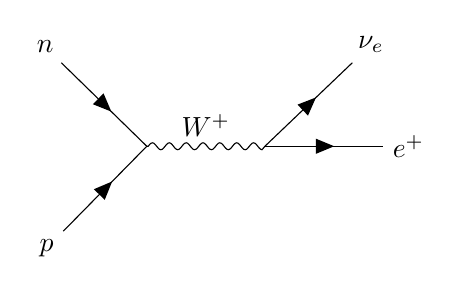
\begin{tikzpicture}
			\begin{feynman}
				\vertex (a);
				\vertex [below left=of a] (proton) {\(p\)};
				\vertex [above left=of a] (neutron) {\(n\)};

				\vertex [right=of a] (b);
				\vertex [right=of b] (electron) {\(e^+\)};
				\vertex [above right=of b] (neutrino) {\(\nu_e\)};


				\diagram* {
				(neutron) -- [fermion] (a),
				(proton) -- [fermion] (a),
				(a) -- [photon, edge label=\(W^+\)] (b) -- [fermion] (electron),
				(b) -- [fermion] (neutrino),
				};
			\end{feynman}
		\end{tikzpicture}

		$p \longrightarrow n + e^+ + \nu_e$
	\end{center}

	\paragraph{Electron Capture}
	\begin{center}
		\feynmandiagram[horizontal=a to b] {
		proton [particle=\(p\)] -- [fermion] a -- [fermion] neutron [particle=\(n\)],
		a -- [boson, edge label=\(W^+\)] b,
		b -- [fermion] neutrino [particle=\(\nu_e\)],
		electron [particle=\(e^-\)] -- [fermion] b,
		};

		$p + e^- \longrightarrow n + \nu_e$
	\end{center}

	\paragraph{Electron-Proton Collision}
	\begin{center}
		\feynmandiagram[horizontal=a to b] {
		proton [particle=\(p\)] -- [fermion] a -- [fermion] neutron [particle=\(n\)],
		a -- [boson, edge label=\(W^-\)] b,
		b -- [fermion] neutrino [particle=\(\nu_e\)],
		electron [particle=\(e^-\)] -- [fermion] b,
		};

		$p + e^- \longrightarrow n + \nu_e$
	\end{center}

	\subsection{Classification of Particles}
	All particles fall into 2 categories: hadrons and leptons. Hadrons consists of
	quarks while leptons are fundamental particles. Leptons cannot interact with the
	strong nuclear force.

	\begin{center}
		\feynmandiagram[layered layout, vertical] {
			a [particle={Particle Classification}] -- b [particle=Hadrons],
			b -- c [particle=Baryons],
			b -- d [particle=Mesons],
			a -- e [particle=Leptons],
		};
	\end{center}

	Baryons consists of any combination of 3 quarks or antiquarks. Mesons consists
	of a quark and an antiquark.
	\medskip

	The classes of particles also have their corresponding antiparticles.
	\begin{align*}
		\text{proton (baryon)}      & \Leftrightarrow \text{antiproton (antibaryon)}  \\
		\text{electron (lepton)}    & \Leftrightarrow \text{positron (antilepton)}    \\
		\text{pion $\pi^+$ (meson)} & \Leftrightarrow \text{pion $\pi^-$ (meson)}     \\
		\text{kaon $K^0$ (meson)}   & \Leftrightarrow \text{kaon $\bar{K}^0$ (meson)}
	\end{align*}

	Pions are exchange particles for the strong nuclear force. Kaons decay into
	pions. The only stable baryon is the proton, every other baryon decays into
	protons.
	\medskip

	Muon are a flavour of lepton, the same classification as electrons. Muon has a
	bigger rest mass than electrons. Muon also decay into electron.

	\subsubsection{Quantum Numbers}
	\paragraph{Baryon}
	Baryon number is the number of baryons in a system minus the number of
	antibaryons. Baryon number is a quantum number, therefore, it is a conserved
	quantity. The number of baryons at an initial state is equal to the number of
	baryons at the end state.
	\medskip

	All baryons have a baryon number of $+1$ and all antibaryon have a baryon number
	of $-1$.
	\begin{align*}
		n                        & \longrightarrow p + e^- +\bar{\nu}_e \\
		\text{baryon number:} +1 & \longrightarrow +1 +0 +0 = 1
	\end{align*}

	\paragraph{Lepton}
	Lepton consists of 3 flavours: electron, muon and tau. The same with quantum
	numbers, the each flavour of lepton number must be conserved in all
	interactions. Each lepton numbers assigns $+1$ to particles and $-1$ for
	antiparticles.
	\begin{align*}
		n                        & \longrightarrow p + e^- +\bar{\nu}_e \\
		\text{lepton number: } 0 & \longrightarrow 0 + 1 - 1 = 0
	\end{align*}

	\paragraph{Strange}
	Strange particles are produced through the strong nuclear interactions and
	decays through the weak nuclear interactions, this happens when kaons
	decay into pions. Strangeness is always created in particle-antiparticle pair.
	Strange quark and antiquark are denoted by $s$ and $\bar{s}$ with strangeness of
	$-1$ and $+1$, respectively. Strangeness is a quantum number and is conserved
	but only through the strong nuclear interactions. In weak interactions,
	strangeness can change into $+1$, $-1$ or $0$.
	\begin{align*}
		K^- + p                     & \longrightarrow \Xi^0 + K^0    \\
		s\bar{u} + uud              & \longrightarrow uss + d\bar{s} \\
		\text{strangeness: } -1 + 0 & \longrightarrow -2 + 1 = -1
	\end{align*}

	In the example, strangeness is conserved, so it must be interacting through the
	strong nuclear force. A pair or strange quark-antiquark is also created in this
	instance.
	\begin{align*}
		K^0                     & \longrightarrow \pi^+ + \pi^-       \\
		d\bar{s}                & \longrightarrow u\bar{d} + d\bar{u} \\
		\text{strangeness: } +1 & \longrightarrow 0 + 0 = 0
	\end{align*}
	In this example, strangeness is not conserved, therefore, the interaction must
	have occurred through the weak nuclear force.

	\subsection{Quarks and Antiquarks}
	Quarks and antiquarks can have the following properties:
	\medskip
	\begin{itemize}
		\item[---] charge
		\item[---] baryon number
		\item[---] strangeness
	\end{itemize}
	\paragraph{Baryon Numbers Explained}
	Baryon number is commonly defined as the number of baryon particles minus the
	number of baryon antiparticles. But, a more in-depth explanation is baryon
	numbers is defined as follows:
	\begin{equation}
		B = \dfrac{1}{3}(n_q - n_{\bar{q}})
	\end{equation}
	The formula equates the baryon number as one-third of the sum of quarks minus
	the antiquarks in a system. The simplified definition for the baryon number is
	generally easier to work with. This explains why quarks and antiquarks can have
	baryon numbers.

	\subsubsection{Common Baryons and Antibaryons}
	\begin{center}
		\begin{tablehere}
			\begin{tabular}{|c|c|}
				\hline
				Baryons     & Quark Composition       \\
				\hline
				Proton      & $uud$                   \\
				Neutron     & $udd$                   \\
				Antiproton  & $\bar{u}\bar{u}\bar{d}$ \\
				Antineutron & $\bar{u}\bar{d}\bar{d}$ \\
				\hline
			\end{tabular}
		\end{tablehere}
	\end{center}

	\subsubsection{Common Mesons}
	\begin{center}
		\begin{tabular}{|c|c|}
			\hline
			Mesons      & Quark Composition \\
			\hline
			$\pi^+$     & $u\bar{d}$        \\
			$\pi^-$     & $d\bar{u}$        \\
			$K^+$       & $u\bar{s}$        \\
			$K^-$       & $s\bar{u}$        \\
			$K^0$       & $d\bar{s}$        \\
			$\bar{K}^0$ & $s\bar{d}$        \\
			\hline
		\end{tabular}
	\end{center}

	\subsubsection{Free Neutron Decay}
	Since proton is the only stable baryon, neutrons can decay into protons. Neutron
	decay only happens when when it is free from a nucleus.

	\begin{center}
		\begin{tikzpicture}
			\begin{feynman}
				\vertex (a);
				\vertex [below left=of a] (neutron) {\(n\)};
				\vertex [above left=of a] (proton) {\(p\)};

				\vertex [right=of a] (b);
				\vertex [right=of b] (electron) {\(e^-\)};
				\vertex [above right=of b] (neutrino) {\(\bar{\nu}_e\)};


				\diagram* {
				(neutron) -- [fermion] (a),
				(proton) -- [fermion] (a),
				(a) -- [photon, edge label=\(W^-\)] (b) -- [fermion] (electron),
				(b) -- [fermion] (neutrino),
				};
			\end{feynman}
		\end{tikzpicture}

		$n^0 \longrightarrow p^+ + e^- + \bar{\nu}_e$
	\end{center}

	\subsection{Application of Conservation Laws}
	All particle interactions must follow the set of conservation laws in order for
	the interaction to be seen as valid. This is due to the general framework of
	quantum physics.

	\subsubsection{Conservation Laws}
	Conservation laws are set of rules that interactions follow. Conservation laws can be split into 2 types: classical quantities and quantum quantities. But, for the sake of simplicity, both will be called conservation laws.
	\medskip

	These are quantities that must be conserved in any interaction:
	\medskip
	\begin{enumerate}
		\item Energy
		\item Momentum
		\item Charge
		\item Baryon number
		\item Electron lepton number
		\item Muon lepton number
		\item Tau lepton number
		\item Strangeness (only in strong interactions)
	\end{enumerate}

	\subsubsection{Change of Quark Character}
	In $\beta^-$ or $\beta^+$ decays, the quark characters, or flavours, can change.
	The change of quark flavour does not violate conservation laws. This also
	applies to any other interactions that change quark characteristics.

	\paragraph{$\beta$ Decay}
	\begin{align*}
		 & \beta^-: udd \xrightarrow{W^-}uud + e^- + \bar{\nu}_e \\
		 & \beta^+: uud \xrightarrow{W^+} udd + e^+ + \nu_e      \\
	\end{align*}
\end{multicols*}
\end{document}
